\section{Спектральный метод решения задачи Коши для систем обыкновенных дифференциальных уравнений посредством  ортогональной в смысле Соболева системы функций, порожденной системой Хаара}

В данном подразделе рассмотрен итерационный метод решения задачи Коши для систем нелинейных дифференциальных уравнений, основанный на использовании ортогональной в смысле Соболева системы функций, порожденной функциями Хаара.

\subsection{Введение}
\label{mmgmsr2-intro}

Рассмотрим задачу Коши для нелинейной системы обыкновенных дифференциальных уравнений вида
\begin{equation}\label{mmgmsr2-cauchy-problem}
y'(x)=f(x,y), \quad y(a)=y^0, \quad x \in [a,b],
\end{equation}
где $f=(f_1, \ldots, f_m)$, $y=(y_1, \ldots, y_m)$. %Здесь и далее жирным шрифтом мы будем обозначать векторные объекты.
Вектор-функцию $f(x,y)$ будем считать непрерывной в некоторой замкнутой  области $\bar G$ переменных $(x,y)$, содержащей точку $(a,y^0)$.
Будем также полагать, что по переменной $y$ функция $f(x,y)$ удовлетворяет условию Липшица
\begin{equation}\label{mmgmsr2-f-lip-cond}
\|f(x,\alpha)-f(x,\beta)\|\le \lambda\|\alpha-\beta\|,
\quad a \le x \le b,
\end{equation}
где $\|(y_1,\ldots,y_m)\|=\sqrt{\sum_{l=1}^my_l^2}$.
Не ограничивая общности, мы можем считать, что  $[a,b] \times \mathbb{R}^m \subset \bar G$, так как в случае необходимости мы всегда можем продолжить функцию $f(x,y)$ по переменной $y$ на всё $\mathbb{R}^m$, сохраняя свойство её подчинённости условию Липшица \eqref{mmgmsr2-f-lip-cond}.

В статье \cite{mmgmsr2-SHII-Demi2017-ODESystems} описан итерационный метод решения задачи Коши вида \eqref{mmgmsr2-cauchy-problem} с помощью представления решения $y(x)$ в виде ряда Фурье
\begin{equation}\label{mmgmsr2-fourier-series-r=1}
y(x) = y(a)+\sum\limits_{k=1}^{\infty}c_{1,k}(y)\varphi_{1,k}(x),
\end{equation}
где $y(a)=y^0$ --- начальное условие задачи Коши, а $c_{1,k}(y)=(c_{1,k}(y_1),\ldots,$$c_{1,k}(y_m))$ --- вектор неизвестных коэффициентов Фурье, которые требуется найти, $\Phi_1=\{\varphi_{1,k}(x)\}$ --- система функций, ортогональных на отрезке $[u,v]$ относительно скалярного произведения типа Соболева
\begin{equation}\label{mmgmsr2-inner-prod}
\langle f,g \rangle =
f(u)g(v)+\int_{u}^{v}f'(x)g'(x)\mu(x)dx.
\end{equation}
В работах Шарапудинова И.\,И. (см., например, \cite{mmgmsr2-SharapudinovMuratova, mmgmsr2-Shii-asymp-demi2016, mmgmsr2-Shii-Gadzhieva2016, mmgmsr2-Shii-matzam2017, mmgmsr2-Shii-Shti-izvvuzov2017, mmgmsr2-Shii-lag-demi2015, mmgmsr2-SHII-MMG-Demi2015}) разработаны теория и методы построения ортонормированных относительно \eqref{mmgmsr2-inner-prod} систем функций.
Для этого выбирается одна из классических систем $\Phi =\{\varphi_k\}_{k=0}^\infty$, ортогональных
относительно обычного скалярного произведения
\begin{equation}\label{mmgmsr2-classic-mul}
\langle f,g \rangle =\int_{u}^{v}f(t)g(t)\mu(t)dt,
\end{equation}
и на её основе строятся функции $\varphi_{1,k}(x)$ посредством равенств
\begin{equation}\label{mmgmsr2-phirk}
\varphi_{1,0}(x) =1, \quad
\varphi_{1,k}(x) =\int\limits_{u}^x\varphi_{k-1}(t)dt, \quad k \ge 1.
\end{equation}
Полученная система функций $\Phi_1=\{\varphi_{1,k}\}_{k=0}^\infty$, как показано в упомянутых выше работах, ортонормирована относительно скалярного произведения \eqref{mmgmsr2-inner-prod}. Системы вида \eqref{mmgmsr2-phirk} называются ортогональными по Соболеву системами, порожденными системой функций $\Phi$.

Суть итерационного метода, предложенного в \cite{mmgmsr2-SHII-Demi2017-ODESystems} (см. также \cite{mmgmsr2-SHII-MMG-Demi2017-CosOde}), заключается в разбиении отрезка $[a,b]$ на подотрезки $\Delta_j=[a+jh,a+(j+1)h]$ длины $h$ и последовательном решении исходной задачи Коши на полученных подотрезках.
При этом за начальное условие задачи (будем обозначать его $y^j$) на отрезке $\Delta_j$, $j>0$, берется значение в точке $a+jh$ приближенного решения, полученного на предыдущем отрезке. Для поиска приближенного решения задачи на отрезке $\Delta_j$:
\begin{equation}\label{mmgmsr2-cauchy-x}
y'(x)=f(x,y(x)), \quad x \in \Delta_j, \quad y(a+jh)=y^j,
\end{equation}
осуществляется перевод этой задачи с помощью линейной замены
\begin{equation*}
x=\frac{t-u}{v-u}h+a+jh
%t=\frac{v-u}{h}\bigl(x-(a+ih)\bigr)+u
\end{equation*}
на отрезок ортогональности $[u,v]$. Если ввести обозначение $\eta(t)=y\bigl(\frac{t-u}{v-u}h+a+jh\bigr)$, то задача \eqref{mmgmsr2-cauchy-x} примет вид
\begin{equation}\label{mmgmsr2-cauchy-problem-eta}
\eta'(t)=\frac{h}{v-u}f\Bigl(\frac{t-u}{v-u}h+a+jh,\eta(t)\Bigr), \quad t \in [u,v], \quad \eta(u)=y^j.
\end{equation}
Построение приближенного решения полученной задачи производится с помощью специальным образом сконструированного оператора $A$, действующего в гильбертовом пространстве $l^m_2$, состоящем из элементов $d=\{d^i,\; i=\overline{1,m}\}$, где $d^i=\{d^i_k\} \in l_2$, с нормой $\|d\|=\Bigl(\sum\limits_{i=1}^m \sum\limits_{k} (d_k^i)^2\Bigr)^{\frac{1}{2}}$.
Оператор $A$ устроен таким образом, что его неподвижной точкой являются коэффициенты Фурье $\mathcal{C}(\eta)=\Bigl\{ \{c_{1,k}(\eta_i), \; k \ge 1 \}, \; i = 1, \ldots, m \Bigr\}$ разложения вида \eqref{mmgmsr2-fourier-series-r=1} решения $\eta(t)$ по системе соболевских функций $\Phi_1=\{\varphi_{1,k}(t)\}$ на отрезке $[u,v]$, т.~е. $A(\mathcal{C}(\eta))=\mathcal{C}(\eta)$.
В связи с этим важным становится вопрос о наличии у оператора $A$ свойства сжимаемости.
Как уже отмечалось \cite{mmgmsr2-SHII-Demi2017-ODESystems}, оператор $A$ можно сделать сжимающим в том случае, когда функции системы $\Phi_1$ обладают следующим свойством:
\begin{equation}\label{mmgmsr2-finite-sum-prop}
\kappa^2=\kappa^2(\Phi_1)=
\sum\limits_{k=0}^{\infty}
\int\limits_{u}^{v}
(\varphi_{1,1+k}(t))^2 \mu(t)dt < \infty.
\end{equation}
Более точно, имеет место следующее неравенство:
\begin{equation*}
\|A\mathcal{C}_1 - A\mathcal{C}_2\|_{l_2^m} \le h \lambda \kappa \|\mathcal{C}_1-\mathcal{C}_2\|_{l_2^m},
\end{equation*}
т. е. оператор $A$ будет сжимающим, если $h \lambda \kappa < 1$, а этого всегда можно добиться за счёт выбора $h$, если $\kappa < \infty$.

Идея построения оператора $A$ основана на следующих соотношениях:
\begin{align}
\label{mmgmsr2-eta-fourier}
\eta(t) = \eta(0)+ &\sum_{k=0}^\infty c_{1,k+1}(\eta) \varphi_{1,k+1}(t),\\
\label{mmgmsr2-eta'-fourier}
\eta'(t) =  &\sum_{k=0}^\infty c_{1,k+1}(\eta)\varphi_k(t),\\
\label{mmgmsr2-q-fourier}
q(t)=
\frac{1}{v-u}f\Bigl(\frac{t-u}{v-u}h+a+jh,\eta(t)\Bigr)
= &\sum_{k=0}^\infty c_{k}(q)\varphi_k(t),
\end{align}
где первое соотношение --- это разложение функции $\eta(t) \in W^1_{L^2_\mu}$ в ряд Фурье по системе $\{\varphi_{1,k}\}$, а второе и третье представляют собой ряды Фурье по системе $\{\varphi_{k}\}$ функций $\eta'(t) \in L^2_\mu$ и $q(t) \in L^2_\mu$ соответственно.
Отметим, что в соотношении \eqref{mmgmsr2-eta-fourier} ряд Фурье сходится равномерно (см., например, \cite[теорема 2]{mmgmsr2-SHII-MMG-Demi2015}), а в \eqref{mmgmsr2-eta'-fourier} и \eqref{mmgmsr2-q-fourier} --- в метрике $L^2_\mu$ (в силу полноты системы $\varphi_{k}$ в пространстве $L^2_\mu$). Из \eqref{mmgmsr2-cauchy-problem-eta}, \eqref{mmgmsr2-eta'-fourier} и \eqref{mmgmsr2-q-fourier} следует
\begin{equation*}
c_{1,k+1}(\eta)=hc_k(q)=
\frac{h}{v-u}
\int_{u}^{v}
f\Bigl(\frac{t-u}{v-u}h+a+jh,\eta(t)\Bigr)
\varphi_k(t)\mu(t)dt,
\end{equation*}
что с учетом \eqref{mmgmsr2-eta-fourier} приводит к соотношению ($k \ge 0$)
\begin{equation*}
c_{1,k+1}(\eta)=
\frac{h}{v-u}\int_{u}^{v}f\Bigl(\frac{t-u}{v-u}h+a+jh,\eta(0)+ \sum_{l=0}^\infty c_{1,l+1}(\eta) \varphi_{1,l+1}(t)\Bigr)\varphi_k(t)\mu(t)dt.
\end{equation*}
Выражение в правой части и представляет собой упомянутый оператор $A$, сопоставляющий точке $\bar{d} \in l^m_2$ точку $\bar{\bar{d}} \in l^m_2$ по следующему правилу
\begin{equation*}
\bar{\bar{d}}^i=
\Bigl\{
\frac{h}{v-u}\int_{u}^{v}f\Bigl(\frac{t-u}{v-u}h+a+jh,\eta(0)+
\sum_{l=0}^\infty \bar{d}^i_l \varphi_{1,l+1}(t)\Bigr)\varphi_k(t)\mu(t)dt,
\: k \ge 0
\Bigr\},
\end{equation*}
где $i=\overline{1,m}$.

\subsection{Численная реализация}
Рассмотрим численную реализацию описанного выше итерационного метода на основе системы $\mathcal{X}$ функций Хаара \eqref{mmgmsr1-haar-def} и порождённой ею по формулам \eqref{mmgmsr2-phirk} системы $\mathcal{X}_1$ функций \eqref{mmgmsr1-inner-prod-gen}.

Искомые коэффициенты $c_{1,k+1}(\eta)$ разложения решения $\eta(t)$ задачи \eqref{mmgmsr2-cauchy-problem-eta} в ряд Фурье --- Соболева вида \eqref{mmgmsr2-fourier-series-r=1}, как это видно из предыдущего пункта, являются неподвижной точкой оператора $A$. Шарапудиновым И.\,И. было показано, что $\kappa(\mathcal{X}_1)=\frac{1}{\sqrt{2}}$, поэтому для заданной правой части $f(x,y)$ при выборе $h<\frac{\sqrt{2}}{\lambda}$ ($\lambda$ --- константа Липшица функции $f(x,y)$) оператор $A$ будет сжимающим. Следовательно, коэффициенты $c_{1,k+1}(\eta)$ можно найти методом простых итераций.

В численной реализации описанного итерационного метода мы будем использовать конечномерный аналог оператора $A$, в котором вместо бесконечной суммы используется частичная сумма порядка $N$:
\begin{equation}\label{mmgmsr2-AN-operator}
A_N(\bar{d})=
\Bigl\{
h\int_{0}^{1}f\Bigl(ht + a + jh,\eta(0)+ \sum_{l=0}^N \bar{d}^i_l \varphi_{1,l+1}(t)\Bigr)\chi_{k}(t)dt,
\: k \ge 1
\Bigr\}_{i=1}^m.
\end{equation}
В данной формуле мы учли, что для системы Хаара вес $\mu(t)=1$ и отрезок ортогональности $[u,v]=[0,1]$. Заметим, что для вычисления значения оператора $A_N$ часто требуется находить значение линейных комбинаций порожденных функций (второй аргумент функции $f$). Для их вычисления мы воспользуемся быстрым алгоритмом, предложенным в предыдущем подразделе. Далее, интеграл в формуле \eqref{mmgmsr2-AN-operator} представляет собой коэффициент Фурье $c_k(q)=c_k(q; \mathcal{X})$ по системе Хаара \eqref{mmgmsr1-haar-def} функции $q(t)=f\Bigl(ht + a + jh,\eta(0)+ \sum_{l=0}^N \bar{d}^i_l \varphi_{1,l+1}(t)\Bigr)$. Для быстрого вычисления коэффициентов с номерами $k=\overline{1,N}$, $N=2^{n_{max}+1}$, мы воспользуемся следующими формулами (см. также \cite[c. 47]{mmgmsr2-bib-farcov}). Введем в рассмотрение следующие вспомогательные величины:
\begin{equation}\label{mmgmsr2-a-coeffs}
a_{n,s} = 2^{n/2} \int_{\Delta^s_{n+1}} q(t)dt, \quad s = \overline{1,2^{n+1}}.
\end{equation}
Поскольку по определению
\begin{equation*}
c_k(q)=c_n^s(q)=2^{n/2}\Bigl(
\int\limits_{\Delta_{n+1}^{2s-1}}q(t)dt-
\int\limits_{\Delta_{n+1}^{2s}}q(t)dt
\Bigr), \quad k=2^n+s, \; s=\overline{1,2^n},
\end{equation*}
то
\begin{equation}\label{mmgmsr2-haar-coeffs-using-a}
c_n^s(q)=a_{n,2s-1}-a_{n,2s},
\quad s = \overline{1,2^{n}}.
\end{equation}
Заметим также, что величины $a_{n-1,s}$ можно выразить через $a_{n,s}$ по формуле:
\begin{equation}\label{mmgmsr2-a-coeffs-recurr}
a_{n-1,s}=\frac{a_{n,2s-1}+a_{n,2s}}{\sqrt{2}},
\quad s = \overline{1,2^{n}}.
\end{equation}
Таким образом, для вычисления коэффициентов с номерами $k=\overline{1,2^{n_{max}+1}}$ мы сначала находим $a_{n_{max},s}$, $s=\overline{1,2^{n_{max}+1}}$ с помощью одной из квадратурных формул. Затем, уменьшая $n$ от $n_{max}$ до $0$, последовательно вычисляем как $a_{n-1,s}$ по формуле \eqref{mmgmsr2-a-coeffs-recurr}, так и коэффициенты $c_n^s(q)$ по формуле \eqref{mmgmsr2-haar-coeffs-using-a}.

%Фрагмент кода, выполняющего основные вычисления, приведен в листинге~\ref{mmgmsr2-lst-HaarSpectralOdeOperator}.

%\begin{longlisting}
%	\caption{Класс HaarSpectralOdeOperator}
%	\label{mmgmsr2-lst-HaarSpectralOdeOperator}
%	\inputminted[mathescape=true, breaklines=true, fontsize={\footnotesize}]{csharp}{code/HaarSpectralOdeOperator.cs}
%\end{longlisting}

%Основной метод класса \textsl{HaarSpectralOdeOperator} --- это !GetValue!, который принимает на вход коэффициенты $\bar{d}$ (в коде используется обозначение !c!) и возвращает коэффициенты $\bar{\bar{d}}=A_N(\bar{d})$.
%Для нахождения коэффициентов !GetValue! использует методы !CalcEta! и !CalcCoeffs!.
%Метод !CalcEta! принимает на вход коэффициенты $\bar{d^i}$ и вычисляет значения частичной суммы $\sum_{j=0}^N \bar{d}^i_j \varphi_{1,j+1}(t)$ (второй аргумент функции $f$ в \eqref{mmgmsr2-AN-operator}, в программе обозначено как !eta!) быстрым алгоритмом, описанным в статье \cite{mmgmsr2-bib-haar-fast-calc}.
%Затем, используя полученные !eta! в методе !CalcCoeffs!, вычисляем коэффициенты $\bar{\bar{d}}$ с помощью алгоритма, описанного выше (см. формулы \eqref{mmgmsr2-haar-coeffs-using-a} и \eqref{mmgmsr2-a-coeffs-recurr}).

\subsection{Компьютерные эксперименты}
Рассмотрим применение приведенной выше программы на нескольких примерах.
\begin{example}\label{mmgmsr2-ex-1}
	Решить задачу Коши
	\begin{equation*}
	\begin{cases}
	y'_1= y_1 - y_2, &\quad y_1(0)=2,\\
	y'_2= -4y_1 + y_2, &\quad y_2(0) = 0, \quad 0 \le x \le 1.
	\end{cases}
	\end{equation*}
\end{example}
Точное решение этой задачи имеет вид: $y_1(x)=e^x$, $y_2(x)=x+e^x$.
При $N=8$ результат выполнения программы для первых 6 итераций приведен на рисунке \ref{mmgmsr2-pic-ex-1}.

\begin{figure}[H]
	\centering
	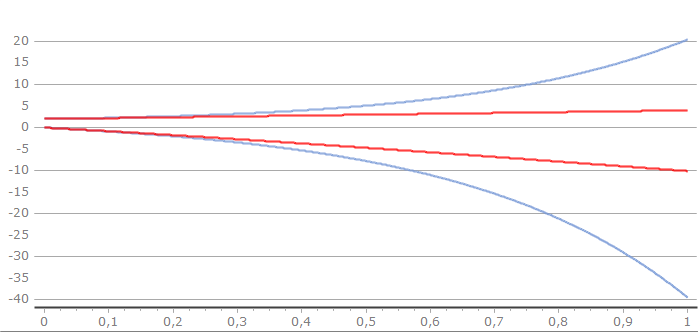
\includegraphics[width=.32\linewidth]{pictures/mmgmsr2-img_1(1)}
	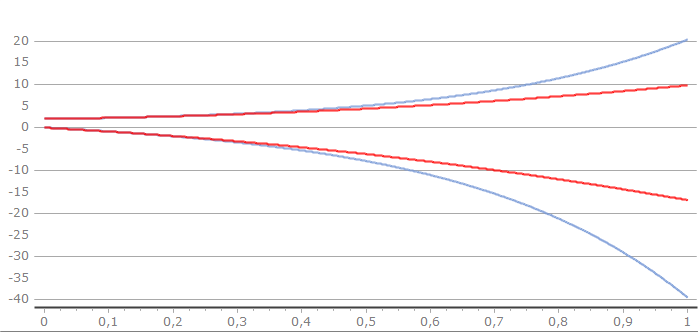
\includegraphics[width=.32\linewidth]{pictures/mmgmsr2-img_1(2)}
	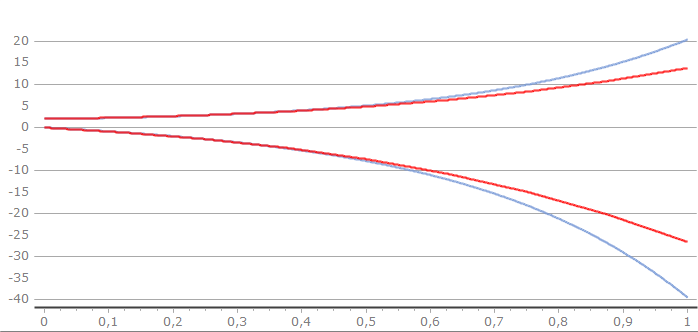
\includegraphics[width=.32\linewidth]{pictures/mmgmsr2-img_1(3)}
	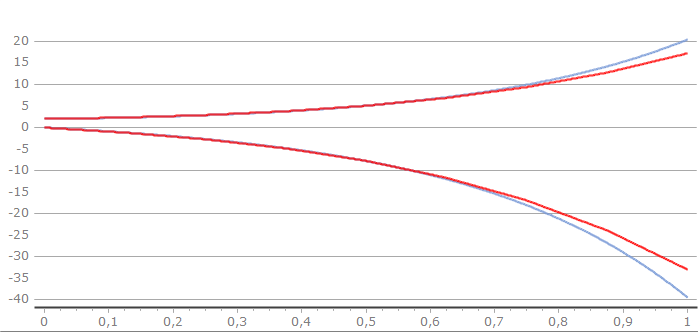
\includegraphics[width=.32\linewidth]{pictures/mmgmsr2-img_1(4)}
	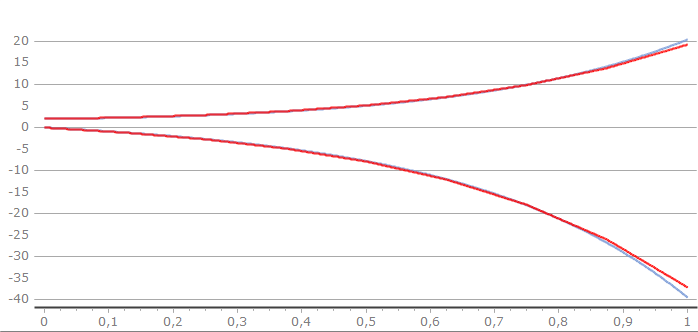
\includegraphics[width=.32\linewidth]{pictures/mmgmsr2-img_1(5)}
	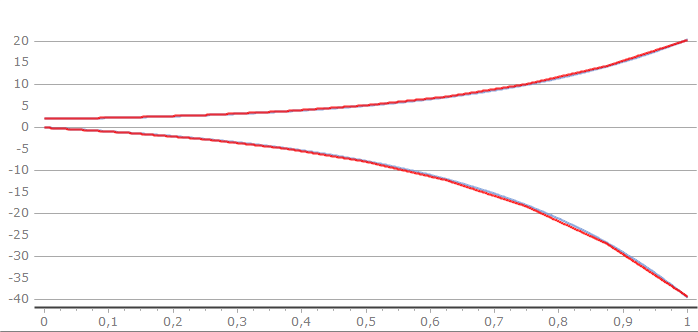
\includegraphics[width=.32\linewidth]{pictures/mmgmsr2-img_1(6)}
	\caption{Первые 6 итераций применения программы к задаче \ref{mmgmsr2-ex-1} (в первой строке итерации 1--3). Синим цветом обозначено точное решение, красным --- его приближение, полученное с помощью программы}
	\label{mmgmsr2-pic-ex-1}
\end{figure}

\begin{example}\label{mmgmsr2-ex-cos}
	Решить задачу Коши
	\begin{equation*}
	\begin{cases}
	y'_1=y_1 - 3 y_2, &\quad y_1(0)=1,\\
	y'_2=3 y_1 + y_2, &\quad y_2(0)=-1, \quad 0 \le x \le \frac{\pi}{2}.
	\end{cases}
	\end{equation*}
\end{example}
Точным решением являются функции $y_1(x)= e^x \cos 3x + \sin 3x$, \\ $y_2(x)= e^x \sin 3x - \cos 3x$.
Результат выполнения программы для первых 6 итераций приведен на рисунке \ref{mmgmsr2-pic-ex-cos}.

\begin{figure}[H]
	\centering
	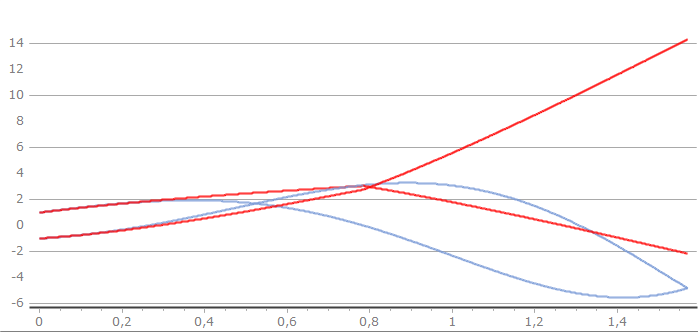
\includegraphics[width=.32\linewidth]{pictures/mmgmsr2-img_2(1)}
	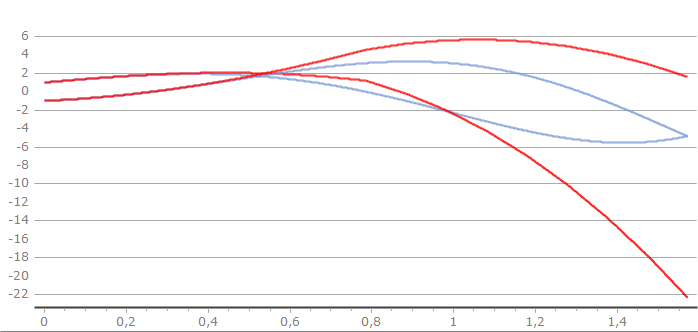
\includegraphics[width=.32\linewidth]{pictures/mmgmsr2-img_2(2)}
	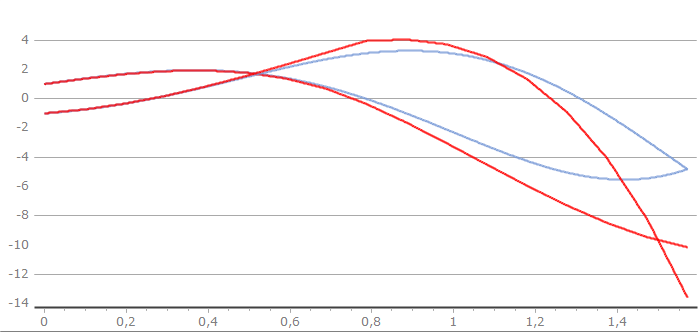
\includegraphics[width=.32\linewidth]{pictures/mmgmsr2-img_2(3)}
	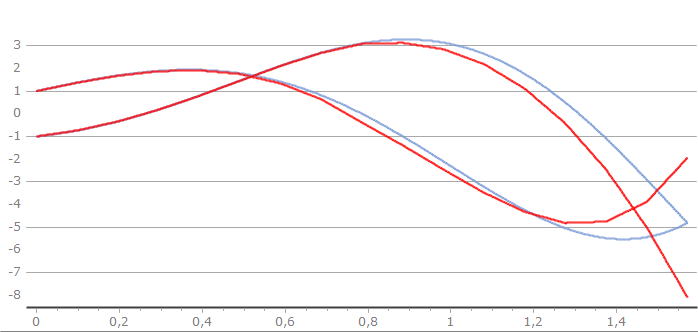
\includegraphics[width=.32\linewidth]{pictures/mmgmsr2-img_2(4)}
	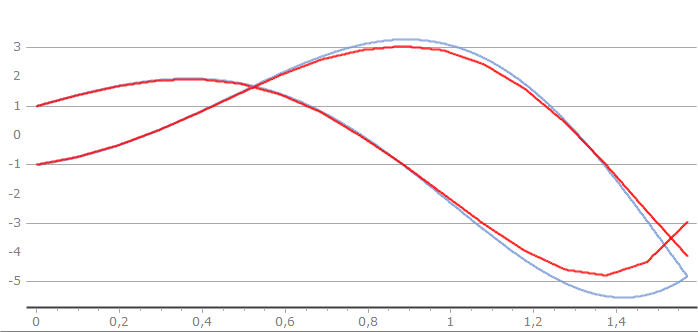
\includegraphics[width=.32\linewidth]{pictures/mmgmsr2-img_2(5)}
	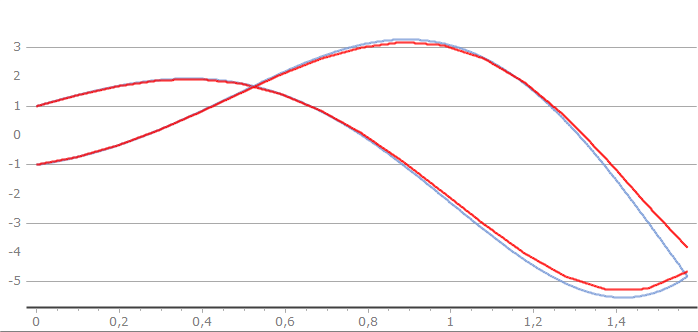
\includegraphics[width=.32\linewidth]{pictures/mmgmsr2-img_2(6)}
	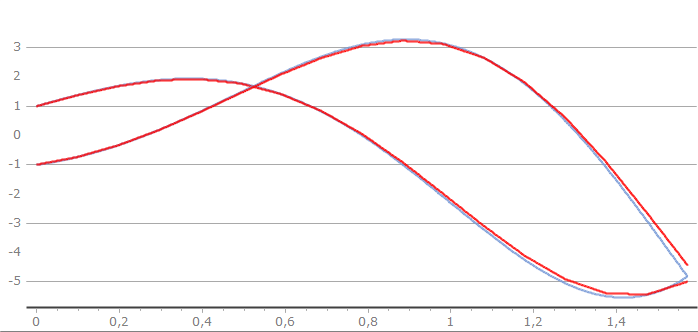
\includegraphics[width=.32\linewidth]{pictures/mmgmsr2-img_2(7)}
	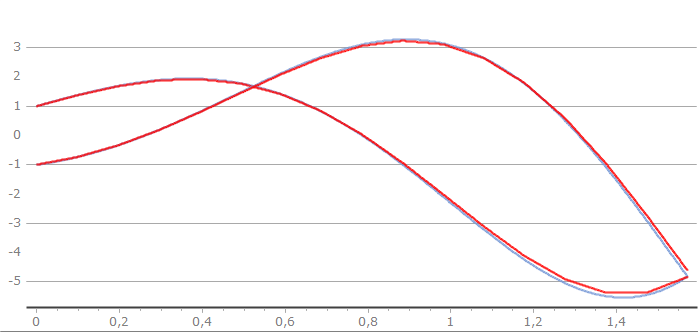
\includegraphics[width=.32\linewidth]{pictures/mmgmsr2-img_2(8)}
	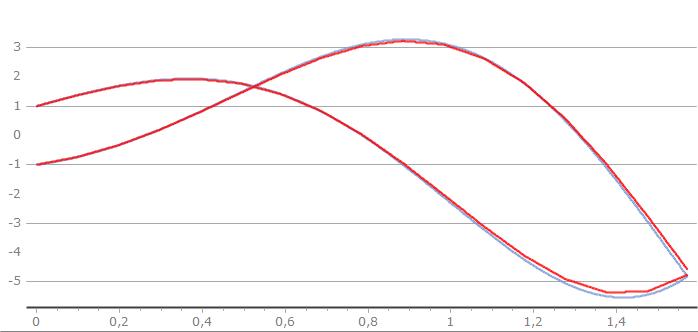
\includegraphics[width=.32\linewidth]{pictures/mmgmsr2-img_2(9)}
	\caption{Первые 9 итераций применения программы к задаче \ref{mmgmsr2-ex-cos} (в первой строке итерации 1--3) при количестве кусков для каждого уравнения равным 2. Синим цветом обозначено точное решение, красным --- его приближение, полученное с помощью программы}
	\label{mmgmsr2-pic-ex-cos}
\end{figure}

\begin{example}\label{mmgmsr2-ex-3}
	Решить задачу Коши
	\begin{equation*}
	\begin{cases}
	y'_1 = y_1 - y_2 - y_3, &\quad y_1(0) = 2,\\
	y'_2 = y_1 + y_2, &\quad y_2(0) = 0,\\
	y'_3 = 3y_1 + y_3, &\quad y_3(0) = -4, \quad 0 \le x \le \frac{\pi}{4}.
	\end{cases}
	\end{equation*}
\end{example}
Точное решение этой задачи имеет вид: $y_1(x)= e^x (2\sin 2x + 2\cos 2x)$, $y_2(x)=e^x (1 - \cos 2x + \sin 2x)$, $y_3 (x) = e^x (-1 - 3\cos 2x + 3\sin 2x)$.
При $N=16$ результат выполнения программы для первых 9 итераций приведен на рисунке \ref{mmgmsr2-pic-ex-3}.

\begin{figure}[H]
	\centering
	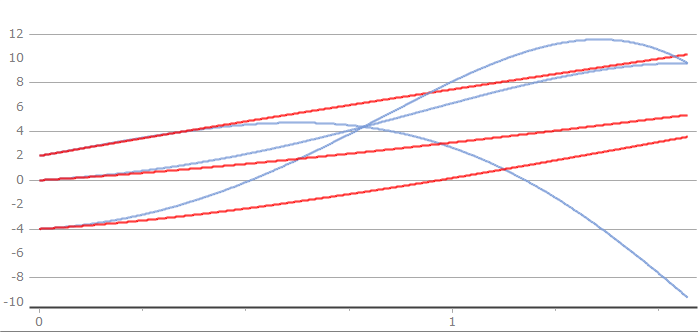
\includegraphics[width=.32\linewidth]{pictures/mmgmsr2-img_3(1)}
	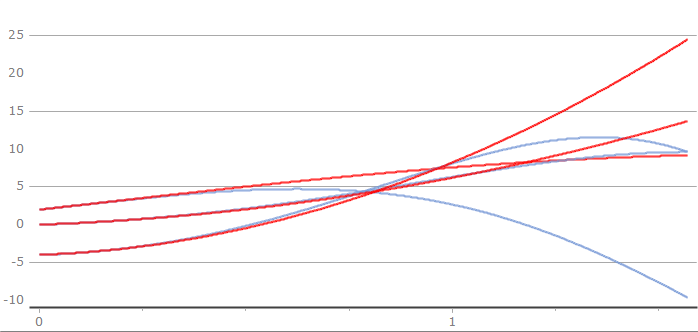
\includegraphics[width=.32\linewidth]{pictures/mmgmsr2-img_3(2)}
	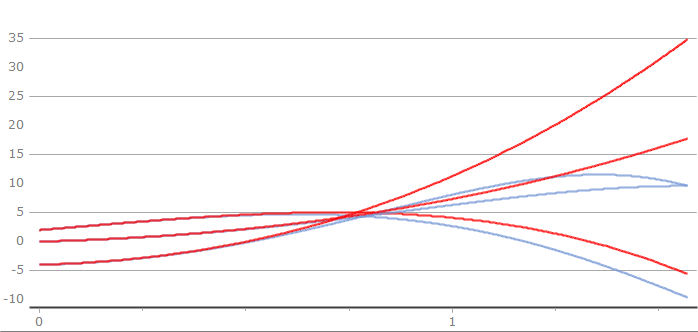
\includegraphics[width=.32\linewidth]{pictures/mmgmsr2-img_3(3)}
	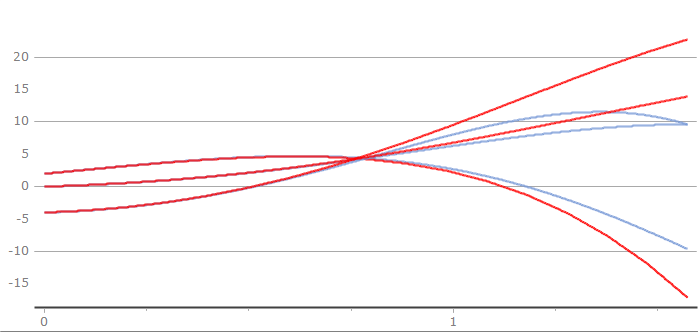
\includegraphics[width=.32\linewidth]{pictures/mmgmsr2-img_3(4)}
	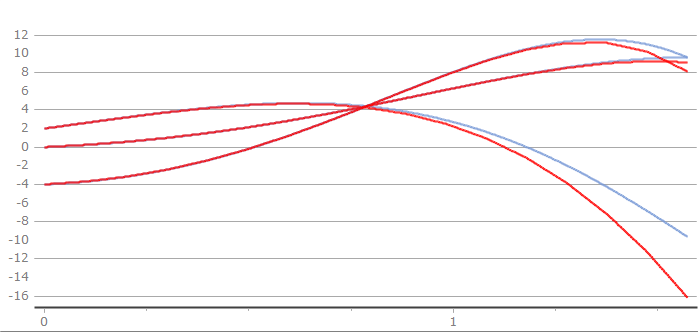
\includegraphics[width=.32\linewidth]{pictures/mmgmsr2-img_3(5)}
	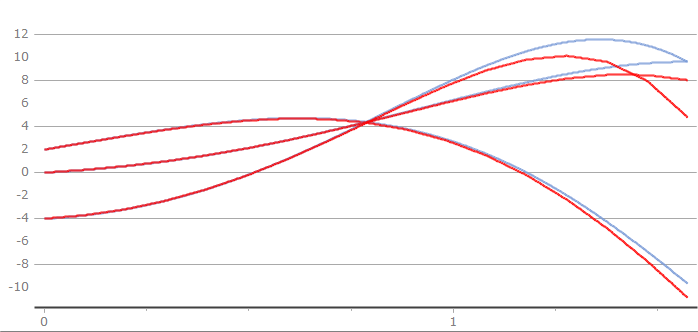
\includegraphics[width=.32\linewidth]{pictures/mmgmsr2-img_3(6)}
	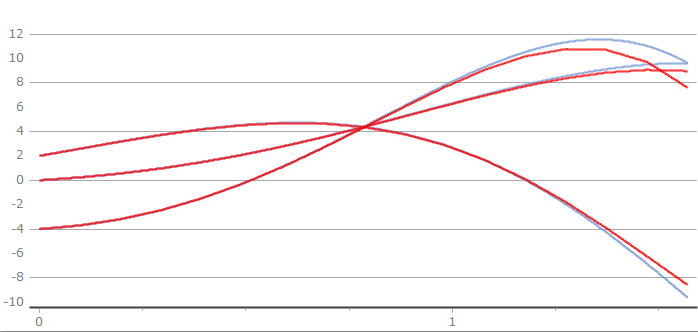
\includegraphics[width=.32\linewidth]{pictures/mmgmsr2-img_3(7)}
	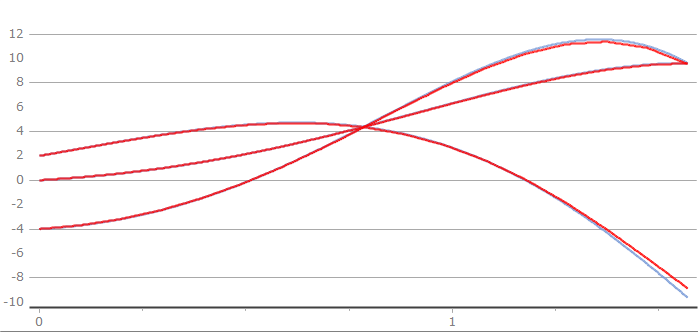
\includegraphics[width=.32\linewidth]{pictures/mmgmsr2-img_3(8)}
	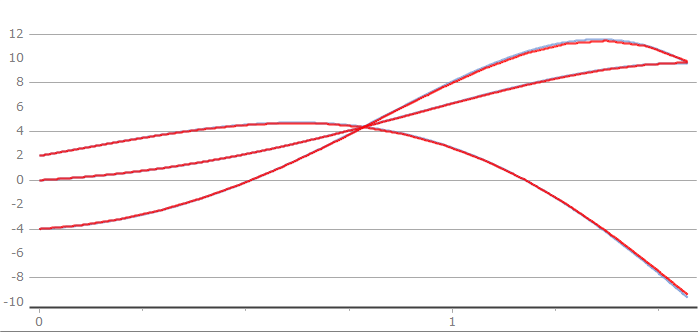
\includegraphics[width=.32\linewidth]{pictures/mmgmsr2-img_3(9)}
	\caption{Первые 9 итераций применения программы к задаче \ref{mmgmsr2-ex-3} (в первой строке итерации 1--3). Синим цветом обозначено точное решение, красным --- его приближение, полученное с помощью программы}
	\label{mmgmsr2-pic-ex-3}
\end{figure}

%\subsection{Заключение}
%
%Рассмотрен итерационный метод решения задачи Коши для систем нелинейных дифференциальных уравнений, основанный на использовании ортогональной в смысле Соболева системы функций, порожденной функциями Хаара. 